

\documentclass[11pt, twoside]{article}
 %\renewcommand{\baselinestretch}{1.0} 
\usepackage{graphicx}

%\usepackage[english,greek]{babel}
%\usepackage{greektex}
\usepackage{amssymb}
\usepackage{amsmath}
\usepackage{amsthm}
%\usepackage{marvosym}


%\usepackage[utf8]{inputenc}
%\usepackage[T1]{fontenc}

%\usepackage[scaled]{helvet}
%\renewcommand\familydefault{\sfdefault} 
%\usepackage[T1]{fontenc}

\usepackage{lmodern}
\usepackage{eurosym}
\usepackage{hyperref}
\hypersetup{colorlinks=true, urlcolor=myblue, citecolor=black, linkcolor=black}

\usepackage[font=small]{caption}

\usepackage[usenames,dvipsnames,svgnames,table]{xcolor}
\usepackage{enumitem}
%\usepackage{float}
\usepackage{color}
\usepackage[top=2cm,bottom=2cm,left=2cm,right=2cm]{geometry}

\usepackage{floatrow}
\usepackage{tcolorbox}
\tcbuselibrary{skins}
\usepackage{lastpage}
\usepackage{tikz}
\usepackage{pgfplots} 
\usetikzlibrary{3d,calc}
\pgfplotsset{compat=newest}
\usetikzlibrary{spy}
\usetikzlibrary{shapes}
\usetikzlibrary{calc}
\usetikzlibrary{shapes.arrows, fadings}
\usetikzlibrary{arrows}
\usetikzlibrary{positioning}
\usetikzlibrary{shadows.blur}
\usetikzlibrary{shapes.symbols}
\usepgfplotslibrary{statistics}



\usepackage{stackengine}


\definecolor{mygreen}{rgb}{0.2,0.55,0.3}
\definecolor{dgreen}{rgb}{0.05,0.6,0.05}
\definecolor{myblue}{rgb}{0.13,0.3,0.55}
\definecolor{myblue2}{rgb}{0.18,0.15,0.40}

\pagestyle{plain}

\let\textacute\'

\newcommand\com[1]{\textcolor{myred}{\textbf{#1}}}

\usepackage{titlesec}
\titlelabel{\thetitle.\quad}

\let\oldsection\section
\renewcommand{\thesubsection}{\arabic{subsection}}
\renewcommand{\thesubsubsection}{\arabic{subsubsection}}



\begin{document}

\definecolor{barblue}{RGB}{153,204,254}
\definecolor{groupblue}{RGB}{51,102,254}
\definecolor{linkred}{RGB}{165,0,33}



\abovedisplayskip=4pt
\abovedisplayshortskip=4pt
\belowdisplayskip=4pt
\belowdisplayshortskip=4pt

\begin{center}
\Large{Sea Turtle Photo-ID Based on Opposite Head Sides}
\end{center}
\vspace{0.3em}

The idea is based on the, so far empirically observed phenomenon, that the similarity of the left and right facial profiles in a given sea turtle individual is higher than than the similarity of (left or right) facial profiles of different individuals. The question is whether (i) this can be quantified and (ii)  can be further exploited to boost the performance of existing state-of-the-art sea turtle photo-ID pipelines.\\

First we would like to quantify this similarity and establish something like the following:

\begin{center}
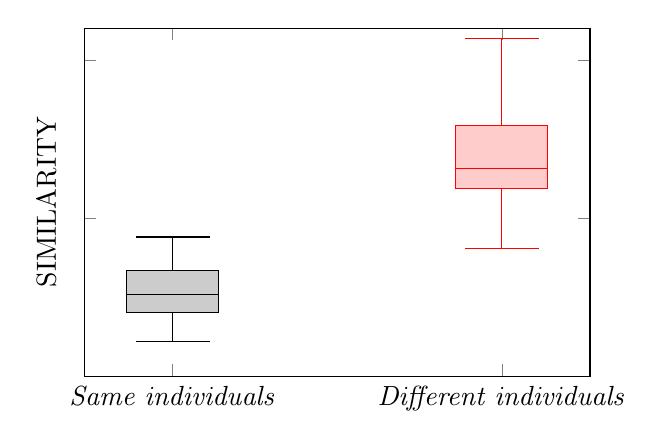
\begin{tikzpicture}
  \begin{axis}
    [
    boxplot/draw direction=y,
        boxplot/variable width,
    boxplot/box extend=0.28,
    ylabel={SIMILARITY},
    height=6cm,
    width=8cm,
    ymin=0,ymax=11,
    cycle list={{black},{red}},
    yticklabels={},
    xtick={1,2},
    xticklabels={\emph{Same individuals}, \emph{Different individuals}}
    ]
    \addplot+[
    fill,fill opacity=0.2,
    boxplot prepared={
      median=2.59,
      upper quartile=3.35,
      lower quartile=2,
      upper whisker=4.4,
      lower whisker=1.1
    },
    ] coordinates {};
    \addplot+[
    fill,fill opacity=0.2,
    boxplot prepared={
      median=6.57,
      upper quartile=7.93,
      lower quartile=5.93,
      upper whisker=10.68,
      lower whisker=4.03
    },
    ] coordinates {};
  \end{axis}
\end{tikzpicture} 
\end{center}

\noindent
\emph{Same individuals}: Denotes pairs of left and right profiles where images of every pair belong to \underline{the same individual}. To avoid cases where the similarity might be due to the same background, lighting conditions etc,  images at every pair should have been taken during a different encounter and ideally using a different camera set up. However one can certainly report results where there no such restrictions on these image pairs and they do have values in certain data collection scenarios.  For instance, during a survey it could happen that one photographs an individual only from the left and a few minutes later it does again so but only from the right.
Another consideration is that  possibly one of the profiles should be flipped so both images have the same orientations, i.e. we want to compare similarity of patterns after one of them has been flipped for consistent comparison. \\
\emph{Different individuals}: Denotes pairs of profiles where images of every pair belong to \underline{different individuals}. By definition here images are taken during different encounters, but distinctions can still be made based on whether images in each pair were taken using the same camera-set up or not etc.\\

\noindent
Thus, perhaps a more detailed version of the previous figure could be something like the following:

\begin{center}
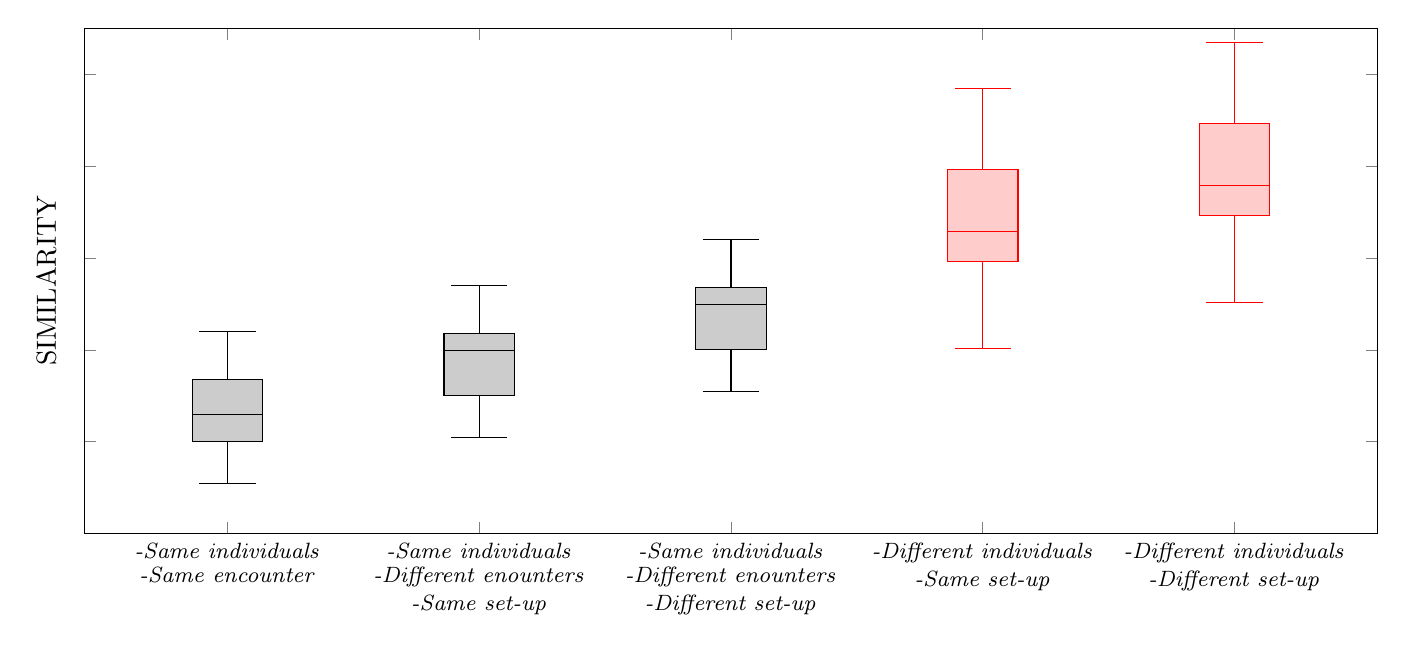
\begin{tikzpicture}
  \begin{axis}
    [
    boxplot/draw direction=y,
    boxplot/variable width,
    boxplot/box extend=0.28,
    ylabel={SIMILARITY},
    height=8cm,
    width=18cm,
    ymin=0,ymax=11,
    cycle list={{black},{black}, {black}, {red}, {red}},
    yticklabels={},
    xtick={1,2, 3, 4, 5},
    xticklabel style   = {align=left, font=\footnotesize},
    xticklabels={\shortstack{\emph{-Same individuals}\\ \emph{-Same encounter}}, 
    \shortstack{\emph{-Same individuals}\\ \emph{-Different enounters} \\ \emph{-Same set-up}},
    \shortstack{\emph{-Same individuals}\\ \emph{-Different enounters} \\ \emph{-Different set-up}},
     \shortstack{\emph{-Different individuals}\\  \emph{-Same set-up}},
     \shortstack{\emph{-Different individuals}\\  \emph{-Different set-up}}
    }
    ]
    \addplot+[
    fill,fill opacity=0.2,
    boxplot prepared={
      median=2.59,
      upper quartile=3.35,
      lower quartile=2,
      upper whisker=4.4,
      lower whisker=1.1
    },
    ] coordinates {};
        \addplot+[
    fill,fill opacity=0.2,
    boxplot prepared={
      median=3.99,
      upper quartile=4.35,
      lower quartile=3,
      upper whisker=5.4,
      lower whisker=2.1
    },
    ] coordinates {};
           \addplot+[
    fill,fill opacity=0.2,
    boxplot prepared={
      median=4.99,
      upper quartile=5.35,
      lower quartile=4,
      upper whisker=6.4,
      lower whisker=3.1
    },
    ] coordinates {};
    \addplot+[
    fill,fill opacity=0.2,
    boxplot prepared={
      median=6.57,
      upper quartile=7.93,
      lower quartile=5.93,
      upper whisker=9.68,
      lower whisker=4.03
    },
    ] coordinates {};
        \addplot+[
    fill,fill opacity=0.2,
    boxplot prepared={
      median=7.57,
      upper quartile=8.93,
      lower quartile=6.93,
      upper whisker=10.68,
      lower whisker=5.03
    },
    ] coordinates {};
  \end{axis}
\end{tikzpicture} 
\end{center}

\noindent
\textbf{Crucial: Was Megadescriptor  trained to have this information already? How could we check this?}\\
Does Megadescriptor (or any model that assigns distances for that matter) have the property that \underline{by design} it assigns higher similarity to profiles of the same individuals no matter whether there are left or right? Thene there would be some danger when performing experiments on the SeaTurtleID2022 dataset which has been seen by the Megadescriptor during training.
We can do one of the following:
\begin{enumerate}
\item Train again from scratch but using only images showing one fixed side for the SeaTurtleID2022 dataset. But maybe too expensive and out of the question...
\item Perform the tests on individuals unseen by the Megadescriptor. That can be new individuals by Kostas, or completely new datasets e.g. Sarah's or from datasets from Kostas' contacts in Reunion Island, Maldives, Egypt etc (mainly Green and Hawksbill turtles).
\end{enumerate}


\noindent
\textbf{Some meaningful experiments...}\\
One simple experiment is to take e.g.\ \underline{all the right profiles} of the SeaTurtleID2022 dataset, train a classifier at a closed-set setting, (this can be either on random or time-aware split; or both) but then \underline{test only with left profiles}. Do we get results that are better than random? Here one should make sure that it is really left vs right, i.e.\ there is essentially no overlap between the profiles, as we want to classifier to judge based on the lateral facial patterns and not based on some overlapping dorsal area (even though even it that happens it has a value!). Again, both random and time-aware splits have value.\\

\noindent
Another relevant experiment, closer to image retrieval and thus closer to the usual proto-ID practice, is to perform experiments where every time a query image is tried to be matched with the closest image of database, but only the opposite side of the query individual is available at the database. \\[0.2em]
\emph{In other words, in the absence of the correct side in the database, will the opposite side be selected instead?}\\[0.2em]
This is very relevant in practice and if it is successful it will attract some attention. It is expected to work if the black and the red boxes of the previous figures are well one above the other.\\

\noindent
\textbf{Regarding existing experiments...}\\
In the ``match same side/match diff side/other/ wrong match experiments'': \\
- It would be interesting to investigate more the "wrong match". How many of those are from the same and how many are from the different side.\\
- For some individuals we might not have more than ``$k$" images so that could contribute to many wrong matches for large $k$.\\
- Maybe having also cumulative results, e.g. ``at least one correct match in the first $k$ outputs''. Perform this both when the opposite side matches are by design forbidden and when they are allowed and quantify how much we gain when they are allowed.\\

\noindent
\textbf{A general question..}\\
In general, how much ``flipping-at-test-time' helps? Experiments with or without flipping...

\end{document}










